\chapter{Quantics Tensor Cross Interpolation}
\label{chap:QTCI}

Cross approximation is a tensor compression technique well-established in the literature \cite{Oseledets2010, Dolgov2020, Savostyanov2011, Savostyanov2014, Fernandez2022, Fernandez2024}. This technique, pioneered by Oseledets \cite{Oseledets2010} and improved by Dolgov and Savostyanov \cite{Dolgov2020}, aims to find a parsimonious interpolation for multi-index tensors with a limited amount of computational resources. Tensor Cross Interpolation (TCI) permitted TT-representations of multivariate functions at a cheaper cost than any SVD based counterpart. Such compressed TT-representations have been used, among other applications, to compute very complex, multi-dimensional integrations, converging better (with no ``sign problem'' \cite{Loh1990}) than standard sampling routines, such as Monte Carlo \cite{Fernandez2022, Dolgov2020}. Ritter and collaborators have improved the already powerful implementations of TCI, targeting stability and discretization issues of the standard routine \cite{Fernandez2024}. This renewed TCI, however, is not free from suboptimalities, especially when trying to target very complex, ``quasi-singular'' type of problems. 

In this chapter, we summarize the basic technical details of the state-of-the-art implementation of cross interpolation for tensors. \prettyref{sec:TCIalgorithm} gives a generic introduction to all the mathematical and technical details of the TCI routine, in order to provide the reader the tools to understand and, through further reading, reproduce the current state of the algorithm. Nonetheless, considering the goal of this work, no particular importance is given to such details, and more focus is instead directed towards the strengths of the TCI algorithm. Section \ref{sec:TCIFallbacks} then shows how a naively modified version of TCI can be tailored to functions with sharply localised structure. Multiple examples are employed for this purpose.

\section{The algorithm}
\label{sec:TCIalgorithm}

The algorithm is a rank-revealing algorithm for decomposing low-rank, high-dimensional tensors into tensor trains/matrix product states (MPS). Hence, its implementation requires two prerequisites: the tensor should be \textbf{compressible}, and the algorithm used for compressing it should be \textbf{rank-revealing}. The properties are defined as follows:

\begin{definition}[Compressible tensor]
	A tensor $\mathcal{T}$ is {\normalfont \textbf{compressible}} or {\normalfont \textbf{low-rank}} if it can be approximated by a Matrix Product State (MPS) with small rank $\chi$.
	\label{def:compresstensor}
\end{definition}

\begin{definition}[Rank-revealing algorithm]
	An algorithm 
	
	\[
		\renewcommand{\arraystretch}{1.1}% a touch of extra vertical room
		\begin{array}{r c >{{}}c<{{}} c} 
		\mathcal{A}: &
		\mathds{K}^{d_1 \times \dots \times d_\mathcal{L}} &
		\longrightarrow &
		\mathds{K}^{d_1 \times \dots \times d_\mathcal{L}} \\[2pt]
		& \mathcal{T} &
		\longmapsto &
		\widetilde{\mathcal{T}}
		\end{array}
	\]

	is said to be {\normalfont \textbf{rank-revealing}}, if it ouputs a low-rank approximation $\widetilde{\mathcal{T}}$ of any compressible $\mathcal{L}$-dimensional tensor $\mathcal{T}$\footnotemark given as input.
	\label{def:rkralg}
\end{definition}

TCI depends on these two properties to provide a competitive numerical approximation technique. Given a tensor $\mT$ with a hidden low-rank structure as input, TCI always provides a compressed representation of it at a \textit{polynomial-scaling} cost in CPU time and memory. Even when the tensor $\mT$ is high rank, TCI is able to output a TT unfolding $\widetilde{\mT}$ (at a slower convergence rate). Before explaining how TCI works, let us first dive into the mathematical tools that supply TCI of this \textit{rank-revealing} and \textit{compression} properties.

\footnotetext{In \prettyref{def:rkralg} we define a tensor $\mathcal{T}$ as an element of the vector space $\mathds{K}^{I_1 \times \dots \times I_\mathcal{L}}$, this is only true if we consider $\mathcal{T}$ an $\mathcal{L}$-dimensional numerical array, as it is for numerics. More generally $\mathcal{T} \in T^p_q(V) = \{t\ |\ t:V^{\otimes q} \otimes  (V^*)^{\otimes p} \longrightarrow \mathds{K} \} $ (where $\mathds{K} = \mathds{R} \vee \mathds{C}$ and $V = \mathcal{H}$ for most applications).}

\subsection{Matrix Cross Interpolation (CI)}
The TCI algorithm bases its implementation on the following statements: \textit{a $M\times N$ matrix of rank $\chi$ can be represented using only $\order(\chi)$ of its entries} and \textit{a compressible (cf. \prettyref{def:compresstensor}) $M\times N$ matrix can be approximated using  $\order(\tchi) \ll MN$ of its entries}.

Let A be a $M \times N$ matrix, we introduce the following notations:
\begin{itemize}
	\item $\mathds{I} = \{1, \dots, M\}$ is the ordered set of all row indices of $A$;
	\item $\mathds{J} = \{1, \dots, N\}$ is the ordered set of all column indices of $A$;
	\item $\mathcal{I} = \{i_1, \dots, i_{\tchi} \} \subseteq \mathds{I}$ and $\mathcal{J} = \{j_1, \dots, j_{\tchi} \} \subseteq \mathds{J}$ are, respectively, subsets of rows and columns indices of $A$.
\end{itemize}
Therefore, in a $\julia$-like fashion\footnotemark   we define 

\footnotetext{From this point onward, we shall consistently use this notation. Slicing notation of the form $A[r_{\text{start}}:r_{\text{start}}, :]$ ($\equiv A_{r,c}$ with $(r,c) \in \{ r_{start},r_{start}+1,\dots, r_{end}\} \times \{1,2, \dots N\}$) will also be employed.}

\begin{equation}
	\begin{alignedat}{3}
		A[\mathds{I}, \mathcal{J}], \qquad A[\mathcal{I}, \mathds{J}], \qquad P = A[\mathcal{I}, \mathcal{J}] 
	\end{alignedat}
\end{equation}
as the submatrices or \textit{slices} containing the intersection elements of $\mathds{I}$ or $\mathcal{I}$ rows and $\mathds{J}$ or $\mathcal{J}$ columns (in particular $A= A[\mathds{I}, \mathds{J}]$). In a matrix Cross Interpolation (CI) context $P = A[\mathcal{I}, \mathcal{J}]$ is the so-called \textit{pivot matrix} and its elements are the \textit{pivots} of the approximation.

The CI formula then reads \cite{Kumar2016}
\begin{gather}
	\label{eq:MCI}
	 A = A[\mathds{I}, \mathds{J}] \approx A[\mathds{I}, \mathcal{J}] P^{-1} A[\mathcal{I}, \mathds{J}], \\
	\hspace{1cm} \begin{tikzpicture}[remember picture,baseline]
		\node[anchor=north west, inner sep=0] 
			 (img) at (0,0){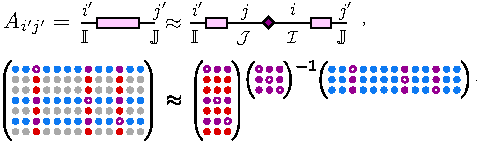
\includegraphics[width=.65\textwidth]{figures/AMCI_IndexSets.pdf}};
		\node[anchor=north east] at (img.north east){\footnotemark};
	\end{tikzpicture}
	\nonumber
\end{gather}
\footnotetext{We introduce here a tensor network diagrammatic representation of the matrix multiplication. The internal connecting solid lines represent summation over the respective matrix indices, according to the \textit{Einstein summation convention}. The external lines represent fixed indices.}
\prettyref{eq:MCI} gives a rank-$\tchi$ approximation of $A$, where $\tchi = \text{dim}\left( \mathcal{I} \right) = \text{dim}\left( \mathcal{J} \right)$. CI is ``only'' a quasioptimal decomposion of $A$ and its accuracy strongly depends on the choice of the pivots; however, contrarily to its optimal counterparts (e.g. SVD), it doesn't require knowing (and saving in memory) the full $M \times N$ matrix to be computed. Moreover, CI correctly represents the rows and column employed to construct of the approximation on the \textit{r.h.s.} of \prettyref{eq:MCI} while also being exact if $\tchi = \chi$. Let's consider the following example: 
\begin{example}[$5 \times 5$ Correlation matrix]
\label{ex:CIcorrmat}
For classical Harmonic Oscillator 1D chain mode-like vectors: 

\[
\begin{alignedat}{2}      
	\boldsymbol{v} = \left(v_1,v_3,\dots,v_5\right) \qquad \boldsymbol{w} = \left(w_1,w_3,\dots,w_5\right)
\end{alignedat}
\]
such that $\boldsymbol{v}\boldsymbol{w}^{T} = 0$, the corresponding position-position correlation matrix can be ``cross interpolated'' as 

\begin{gather}
	\begin{aligned}
		 &C  \;=\; \sigma^2 \boldsymbol{v}^T \boldsymbol{v} + \tilde{\sigma}^2 \boldsymbol{w}^T\boldsymbol{w} = \\[2em]
		&=
		\begin{tikzpicture}[baseline=-0.5ex,
			every node/.style={inner sep=1pt,font=\small}]
			\matrix (M) [matrix of math nodes,
  %––– default: narrow columns –––
  nodes     = {text width=1cm, align=center, minimum height=2em, anchor=center},
  %––– wide columns (1, 3, 5) –––
  column 1/.style = {nodes={fill=red!30 , text width=2.5cm}},
  column 3/.style = {nodes={text width=2.5cm}},
  column 5/.style = {nodes={fill=red!30, text width=2.5cm}},
  %––– coloured rows / corners –––
  row 1/.style          = {nodes={fill=yellow!30}},
  row 5/.style          = {nodes={fill=yellow!30}},
  row 1 column 1/.style = {nodes={fill=orange!30}},
  row 1 column 5/.style = {nodes={fill=orange!30}},
  row 5 column 1/.style = {nodes={fill=orange!30}},
  row 5 column 5/.style = {nodes={fill=orange!30}},
  left delimiter={[}, right delimiter={]},
  ampersand replacement=\&
]{
	\sigma^{2}v_1v_1+ \tilde\sigma^{2}w_1w_1 \& \cdots
				\& \sigma^{2}v_1v_j+ \tilde\sigma^{2}w_1w_j
				\& \cdots
				\& \sigma^{2}v_1v_5+ \tilde\sigma^{2}w_1w_5\\
				 {} \& \ddots
				\& 
				\& \&{}\\
				\vdots \& {}
				\& \sigma^{2}v_iv_j+ \tilde\sigma^{2}w_iw_j
				\& {}
				\& \vdots \\
				{} \&  \& 
				\& \ddots
				\& {}\\
				 \sigma^{2}v_5v_1+ \tilde\sigma^{2}w_5w_1 \& \cdots \& \cdots \& \cdots
				\& \sigma^{2}v_5v_5+ \tilde\sigma^{2}w_5w_5\\
				};
			\draw [decorate, line width=1.5pt,
				decoration = {calligraphic brace,mirror,raise=5pt, amplitude=5pt}] (M.south west) --  (M.south east) node[pos=0.5, below=12pt]{\normalsize $5 \times 5$};
		\end{tikzpicture}
	\end{aligned}
	 \\[1.2em]
	 \nonumber
	 \hspace*{-0.6cm}%
	  \approx
	   \underbrace{%
	  C[\mathds{I} , \mathcal{J}]}_{\displaystyle 5 \times 2}
	\,
	\underbrace{%
	  \left[ \begin{array}{>{\columncolor{orange!30}}c>{\columncolor{orange!30}}c}
		\sigma^{2}v_1v_1+ \tilde\sigma^{2}w_1w_1 & \sigma^{2}v_1v_5+ \tilde\sigma^{2}w_1w_5 \\[0.2em]
		\sigma^{2}v_5v_1+ \tilde\sigma^{2}w_5w_1 & \sigma^{2}v_5v_5+ \tilde\sigma^{2}w_5w_5
	  \end{array}\right]^{-1}}_{\displaystyle 2 \times 2}
	  \,
	  \underbrace{%
	  C[\mathcal{I} , \mathds{J}]}_{\displaystyle 5 \times 2} 
\end{gather}
with $\sigma$ and $\tilde{\sigma}$ the variances of the two modes and $\mathcal{I} = \{ 1,5\}$ and $\mathcal{J} = \{ 1,5\}$. From the definition of $C$ we can recognize that $\rank{C} = 2$. This property is correctly highlighted by its CI decomposition ($\dim \mathcal{I} = \dim \mathcal{J} = 2$), since, in this particular case, the approximation is exact (cf. \prettyref{prop:CI}.\hyperlink{cond:rankexact}{3}). The total number of floating point numbers necessary to store the whole matrix in memory is $5 \times 5 = 25$, while for the CI decomposition $5\times 2 \times 2 + 2\times 2 = 24$ are sufficient. It is easy to deduce that the reduction in memory costs becomes more important for modes of generic dimension $N$ ($N\times N \gg N \times 2 \times 2 + 2\times 2$ when $N \gg 1$).
\end{example}

From the example above we can evince the computational advantage of CI, however -- in order to make such approximation computationally feasable -- some sort of error control is necessary. 
In particular, the error of the CI approximation is related to the \textit{Schur complement} of the matrix \cite{Golub96}. 

\begin{definition}[Schur Complement]
	Let us block partition a matrix $A\in\mathds{K}^{M\times N}$ ($\mathds{K} = \mathds{R}, \mathds{C}$) as follows: 

	\begin{equation}
		\begin{bNiceMatrix}[last-row, last-col]
			A_{11} & A_{12} & {\scriptstyle \tchi} \\
			A_{21} & A_{22} & {\scriptstyle M - \tchi} \\
			{\scriptstyle \tchi} & {\scriptstyle N - \tchi}
		\end{bNiceMatrix}.
	\end{equation}
The {\normalfont \textbf{Schur complement}} $[A/A_{11}]$ of $A$ is defined by 
	\begin{equation}
		\label{eq:Schurcomp}
		[A/A_{11}] = A_{22} - A_{21}(A_{11})^{-1}A_{12}.
	\end{equation}
\end{definition}

\begin{proposition}
	\label{prop:CI}
	The following properties hold for a rank-$\tchi$ Cross Interpolation decomposition of a matrix $A$: 

	\begin{enumerate}
		\item \hypertarget{cond:Schurerr}the error of CI is given by the Schur complement to the pivot matrix;
		\item the approximation is exact for any $i \in \mathcal{I}$ or $j \in \mathcal{J}$; 
		\item \hypertarget{cond:rankexact} the approximation is exact if $A$ has rank $\tchi$.
	\end{enumerate}
	 
\end{proposition}\vspace{-10pt}
\begin{proof}
	\textit{1.-2.} - The Schur complement is invariant under rows and/or column permutations, therefore let us rearrange $A = A[\mathds{I}, \mathds{J}]$ such that
	\begin{equation*}
		A = \begin{bmatrix}
			A[\mathcal{I}, \mathcal{J}] & A[\mathcal{I}, \mathds{J} / \mathcal{J}] \\
			A[\mathds{I} / \mathcal{I}, \mathcal{J}]  & A[\mathds{I} / \mathcal{I}, \mathds{J} / \mathcal{J}]  
		\end{bmatrix}.
	\end{equation*}
Then, the r.h.s. of \prettyref{eq:MCI} can be rewritten as 
	\begin{equation*}
		\tilde{A} = \begin{bmatrix}
			A[\mathcal{I}, \mathcal{J}] & A[\mathcal{I}, \mathds{J} / \mathcal{J}] \\
			A[\mathds{I} / \mathcal{I}, \mathcal{J}]  &   A[\mathds{I} / \mathcal{I}, \mathcal{J}] \left(A[\mathcal{I}, \mathcal{J}] \right)^{-1} A[\mathcal{I}, \mathds{J} / \mathcal{J}]
		\end{bmatrix}
	\end{equation*}
	which gives (cf. Ref. \cite{Fernandez2024})
	\begin{equation}
		A - \tilde{A} = \begin{bmatrix}
			0 & 0 \\
			0 & [A/A[\mathcal{I}, \mathcal{J}]]
		\end{bmatrix}
	\end{equation}
\textit{3.} - If $\rank{A} = \tchi$ and $P = A[\mathcal{I},\mathcal{J}]$ is non-singular, then 

\begin{equation}
	\begin{bmatrix}
		A[\mathcal{I}, \mathcal{J}] & A[\mathcal{I},j] \\
		A[i, \mathcal{J}] & A[i,j]
	\end{bmatrix}\qquad \forall\; (i,j) \in \mathds{I} / \mathcal{I} \times \mathds{J} / \mathcal{J}
\end{equation}
is singular, which gives $ A[i,j] = A[i, \mathcal{J}] \left( A[\mathcal{I}, \mathcal{J}] \right)^{-1} A[\mathcal{I},j]$ $\forall\; (i,j) \in \mathds{I} / \mathcal{I} \times \mathds{J} / \mathcal{J}$(cf. App A-B in Ref. \cite{Fernandez2022}). 
\end{proof}

\prettyref{prop:CI}.\hyperlink{cond:rankexact}{1} underlines the importance of the choice of the pivots and of the pivot matrix, specifically with the purpose of minimizing the Schur complement $[A/A[\mathcal{I}, \mathcal{J}]]$. Such procedure is equivalent to maximising $\det{A[\mathcal{I}, \mathcal{J}]}$ and is known as the \textit{maximum volume principle} \cite{Goreinov1997}. Moreover, from this analysis, we can also get an intuition about why the CI approximation error is at most $O(\tchi^2)$ times the optimal one (e.g. $\tchi$-truncated SVD error) \cite{Schneider2010}, while requiring only subparts of the original matrix to be known. 

\subsubsection{Partial rank-revealing LU decomposition (prrLU)}
Matrix Cross Interpolation presents itself as a very useful tool when it comes to numerical compression of matrices. Generalization of CI to continuous domains \cite{Schneider2010, Fernandez2022} even allows for reduction of numerical complexity of two-dimensional integration and derivation. Nonetheless, for practical, very complex, calculations, CI starts to fail. Numerical instability issues like rounding errors, ill-conditioning or overflowing \cite{Golub96} naturally emerge when CI requires large values of $\tchi$ to be accurate, therefore making the pivot matrix \textit{almost singular}. 

Partial rank-revealing LU (prrLU) \cite{Golub96, Pan2000} matrix decomposition solves many of the numerical fragilities of CI. The prrLU provides a more stable, but equivalent approximation of our matrix to decompose. prrLU avoids any inversion of the pivot matrix $A[\mathcal{I}, \mathcal{J}]$, whereas still requires a small subset of matrix's elements to be known. 

We may summarize the main features of prrLU as follows:

\begin{itemize}
	\item prrLU is \textit{rank revealing}, i.e. it allows for the iterative determination of the rank of the decomposed matrix;
	\item prrLU is \textit{partial} (and therefore \textit{controllable}), i.e. the decomposition is stopped after constructing the first $\tchi$ rows of $L$ and columns of $U$, for a fixed $\tchi$;
	\item prrLU is \textit{updatable}, i.e. given pivot lists $\mathcal{I}, \mathcal{J}$ yielding an approximation $\tilde{A}$ of $A$, new rows and columns can easily be added to $\mathcal{I}, \mathcal{J}$ for an improved approximation. 
\end{itemize}

The prrLU implementation relies on the following LU decomposition (easily inferred from \prettyref{eq:Schurcomp}):

\begin{gather}
	\label{eq:SchurLU}
	\begin{bmatrix}
	A_{11} & A_{12} \\
	A_{21} & A_{22}
	\end{bmatrix}
	%\nonumber \\
	=
	\begin{bmatrix}
	L_{11} & 0 \\
	L_{21} & \identity_{22}
	\end{bmatrix}
	\begin{bmatrix}
	A_{11} & 0 \\
	0 & [A / A_{11}]
	\end{bmatrix}
	\begin{bmatrix}
	U_{11} & U_{12} \\
	0 & \identity_{22}
	\end{bmatrix}\\[6pt]
	\nonumber L_{11} = U_{11} = \identity_{11}, \qquad L_{21} = A_{21}A^{-1}_{11}, \qquad U_{12} = A^{-1}_{11}A_{12}
\end{gather} 
Although matrices $L_{21}$ and $U_{12}$ in \prettyref{eq:SchurLU} contain the inverse of the matrix block $A_{11}$, the state-of-the-art implementation of prrLU limits $A_{11}$ to a $1\times1$ slice; hence, no actual matrix inversion is computed directly! The general prrLU algorithmic routine proceeds as outlined below \cite{Fernandez2024}:  

\vspace{1.5\baselineskip}
\begin{algorithm}[H]
	\caption{Partial rank revealing LU}
	\label{alg:prrLU}
    \SetKwFunction{findBestPivot}{findBestPivot}
	\SetKwFunction{LowerTriangular}{LowerTriangular}
	\SetKwFunction{strictlyUpperTriangular}{strictlyUpperTriangular}
    \SetKwInOut{KwIn}{Input}
    \SetKwInOut{KwOut}{Output}

    \KwIn{$A\in\mathds{K}^{M\times N}$ matrix, maximum rank $\tchi$ and tolerance $\varepsilon$. }
    \KwOut{Rows permutation $\Pi_r$, columns permutation $\Pi_c$, $L$, $U$, $N_{pivots}$}

    $\Pi_r\leftarrow(1,\dots,M)$,\quad $\Pi_c\leftarrow(1,\dots,N)$,\quad 
	$n\leftarrow0$,\quad $\varepsilon_{LU} \leftarrow \varepsilon$\;

	\While{$n<\min(\tchi,\,M,\,N)$}{
		$n\leftarrow n+1$\;
		$(r^\star,c^\star)\leftarrow 
		\findBestPivot\!\bigl(A[n\!:\!N, n\!:\!M]\bigr)$\tcp*[f]{current positions}\;
		swap rows $n\leftrightarrow r^\star$ in $A$ and $\Pi_r$\;
		swap cols $n\leftrightarrow c^\star$ in $A$ and $\Pi_c$\;
		$\varepsilon_{LU} \leftarrow |A_{n,n}|$\;
		\If(\tcp*[f]{error test}){$n>0$ \KwSty{and} $\varepsilon_{LU} <\varepsilon$}{
			\textbf{break}\;
		}	
	}
	
	$L\leftarrow\LowerTriangular\bigl(A[:,\,1\!:\!n]\bigr)$\;
	$U\leftarrow\strictlyUpperTriangular\bigl(A[1\!:\!n,\,:]\bigr)$\;
	\Return{$(\Pi_r,\,\Pi_c,\,L,\,U,\,n)$}\;
\end{algorithm}
\vspace{2\baselineskip}
By iteratively applying \prettyref{eq:SchurLU} on the lower-right block of the internal matrix \(\scriptstyle \begin{bmatrix} A_{11} & 0 \\
	0 & [A / A_{11}] \end{bmatrix}\), while limiting $A_{11}$ to a $1\times 1$ submatrix at each step, \prettyref{alg:prrLU} allows us to obtain an approximation of the form 

\begin{equation}
	A = LDU + \begin{bmatrix}
		0 & 0\\
		0 & [A/A[\mathcal{I}, \mathcal{J}]]
	\end{bmatrix} = \tilde{A} + \textrm{err.},
	\label{eq:prrLUCI}
\end{equation}
equivalent to \prettyref{eq:MCI} (cf. Ref. \cite{Fernandez2024}). In \prettyref{eq:prrLUCI}  $D$ is a diagonal matrix containing -- after iterative permutations --  $\tchi$ pivots of $A$. 
Some remarks about \prettyref{alg:prrLU} are in order
\begin{itemize}
	\item \texttt{findBestPivot}, \texttt{LowerTriangular} and \texttt{strictlyUpperTriangular} are merely renamed counterparts of the $\julia$ routines used in the prrLU implementation of Ref. \cite{Fernandez2024,TensorCrossInterpolation.jl}. The first routine proposes a suitable pivot for the current iteration (often one among several equally valid options), while the latter two return, respectively, the lower-triangular portion and the strict upper-triangular portion of the input matrix.
	\item The implementation of prrLU is based upon the search of a good \textit{pivot} (\texttt{findBestPivot}). Following the \textit{maxvol principle}, a good pivot is defined as one that attempts to maximise the volume of the submatrix $A[\mathcal{I}, \mathcal{J}]$ ($\equiv A_{11}$ after permutations). Hence, the iterative application of \prettyref{eq:SchurLU} reduces the optimal pivot to the largest element of the submatrix $A[n\!:\!N,n\!:\!M]$ at iteration $n$. Such iterative approach, however, does not necessarily extract the pivot matrix $A[\mathcal{I}, \mathcal{J}]$ with larger determinants. This is due to the facto that maximum volume submatrices of larger sizes are not guarantedeed to contain the maximum volume submatrices for smaller sizes. Nonetheless, the algorithm attempts to reach the ideal configuration for $A[\mathcal{I}, \mathcal{J}]$, often with great success. 
	\item Different strategies can be implemented for pivot searching; a naive approach consists in a \textit{full search} scheme scanning the entire submatrix $A[n\!:\!N,n\!:\!M]$. \textit{Rook search} \cite{Poole2000} and \textit{block rook search} \cite{Fernandez2024} are cleverer and cheaper approaches, with comparable robutstness and convergence features, but reduced computational cost $\order(\max\left(M,N\right))$.  
	\item The matrix elements explored during \textit{rook search} are sufficient to perform prrLU of $A$. Therefore, prrLU yields compressibility traits similar to those of CI (see Example \ref{ex:CIcorrmat}). For this reason, prrLU can also be applied to 2-dimensional continuous functions discretized on a grid, whose full structure is uknown a priori. 	
	\item The absolute error of the prrLU approximation is reduced to the modulus of the last inserted pivot, as one can understand from \prettyref{alg:prrLU}. The reason behind this is that we intend to minimize $\parallel\! A - \tilde{A}\!\parallel_{\infty} = \parallel\![A/A[\mathcal{I}, \mathcal{J}]] \!\parallel_{\infty}$ which is bounded by $\parallel\! A[n\!:\!N, n\!:\!M]\!\parallel_{\infty}$ at iteration step $n$.  
\end{itemize}


\subsection{Tensor Cross Interpolation}

Tensor Cross Interpolation is a generalization of matrix Cross Interpolation -- and therefore prrLU (see \prettyref{eq:prrLUCI}) -- to $\mathcal{L}$-dimensional tensors $\mathcal{T}$. Similarly to prrLU, TCI progressively uncovers the \textit{low rank} structure of a given tensor, ultimately rendering a compressed approximation of the input. The main difficulty in the implementation of TCI revolves around bookkeeping of tensor indices -- the \textit{pivots} -- necessary for a correct approximation. 
Hence, let us introduce some useful notation: 
\begin{itemize}
	\item $\mathcal{T}_{\boldsymbol{\sigma}} \in \mathds{K}^{d_1\times d_2\times \dots \times d_\mathcal{L}}$ is the TCI input tensor, with indices $\bsigma \in I_1\times I_2\times \dots \times I_\mathcal{L} := \text{Ind}\left(\mT\right)$ ($|I_i| = d_i\, \footnotemark$); $\mathcal{\widetilde{T}}_{\boldsymbol{\sigma}} \in \mathds{K}^{d_1\times d_2\times \dots \times d_\mathcal{L}}$ is the resulting interpolated tensor:
	\footnotetext{For most application $d_i=d\; \forall i$, with fixed $d$. }
	\begin{align}
		\label{eq:globTTensor}   
	 \mathcal{T}_{\bsigma}
	 = \raisebox{-5mm}{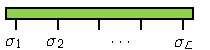
\includegraphics{figures/fnatural_short.pdf}} \approx  \mathcal{\widetilde{T}}_{\boldsymbol{\sigma}} \, ; 
	 \end{align}
	\item $\mathds{I}_\ell = I_1\times I_2\times \dots \times I_\ell$ and $\mathds{J}_\ell = I_\ell\times I_2\times \dots \times I_\mathcal{L}$\footnotemark\; denotes, respectively, the set of all \textit{row multi-indices} and \textit{column multi-indices} up to and from site $\ell$ (e.g. $i_\ell \in \mathds{I}_\ell$, $j_\ell \in \mathds{J}_\ell$ implies $i_\ell = (\sigma_1, \dots, \sigma_\ell)$, $j_\ell = (\sigma_\ell, \dots, \sigma_\mathcal{L})$);
	\item $\mathcal{I}_\ell \subseteq \mathds{I}_\ell$ and $\mathcal{J}_\ell \subseteq \mathds{J}_\ell$ are, respectively, lists of \textit{pivot rows} and \textit{pivot columns} and contain only a subset of the total row and column multi-indices, the \textit{pivots};
	\item the following objects represent \textit{slices} of the original tensor:
	\vspace{.5\baselineskip}
	\begin{gather}
		\nonumber [P_\ell]_{ij} = \mathcal{T}_{i\oplus j} 
		= \raisebox{-5mm}{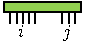
\includegraphics{figures/PtensorWithLegsNoell.pdf}} \, , \quad [T_\ell]_{i\sigma j} \equiv \mathcal{T}_{i\oplus (\sigma) \oplus j} 
		= \raisebox{-5mm}{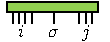
\includegraphics{figures/TtensorWithLegsNoell.pdf}} \, ,\\[6pt] 
		[\Pi_\ell]_{i\sigma \sigma'j} \equiv  \mathcal{T}_{i\oplus (\sigma,\sigma') \oplus j}
	= \raisebox{-5mm}{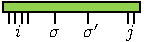
\includegraphics{figures/PiTensorWithLegsNoell.pdf}} \, ,
	\label{eq:Tslices} 
	\end{gather}
	where $\oplus$ is the index \textit{concatenation operation}, i.e. $i\oplus j \equiv (\sigma_1, \dots, \sigma_\mathcal{L})$, for fixed $i\in \mathds{I}_\ell$ and $j \in \mathds{J}_{\ell+1}$. 

\end{itemize}

\footnotetext{$\mathds{I}_\mathcal{L} = \mathds{J}_1$ corresponds to the full set of tensor indices, i.e. $\boldsymbol{\sigma} \in  \mathds{I}_\mathcal{L} = \mathds{J}_1\; \forall \boldsymbol{\sigma}$}

The main purpose of TCI is perform the decomposition of a given tensor using only few elements of (few calls to) the tensor $\mathcal{T}_{\boldsymbol{\sigma}}$. \prettyref{fig:TCIalg} below summarizes the main steps 
of the TCI routine. 

\begin{figure}[htbp]
	\centering
	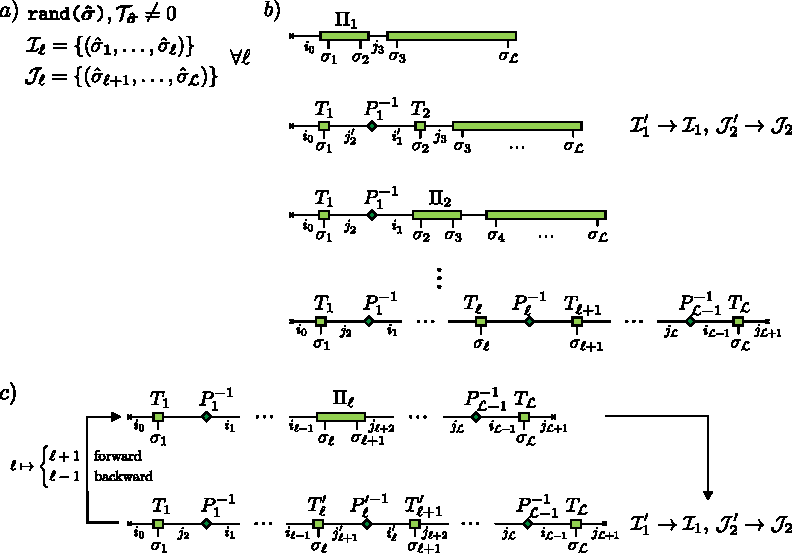
\includegraphics[width=\textwidth]{figures/TCI.pdf}
	\caption{Main steps of the TCI algorithm. $a)$ A set of indices such that $\mathcal{T}_{\hat \sigma} \neq 0$ is chosen randomly from the configuration space $\text{Ind}\left(\mT\right)$. Pivot lists are constructed from the initial multi-indices set. $b)$ A first sweep is performed for an initial Matrix Product State representation of our tensor $\mathcal{T}$. At sites $\ell$ and $\ell+1$, $\Pi_\ell$ tensor slices of the form in \prettyref{eq:Tslices} are constructed from the initial pivot lists $\mathcal{I}_{\ell-1}$ and $\mathcal{J}_{\ell+2}$. prrLU is then perfomed on the ``matricized'' version of $\Pi_\ell$, namely $\bigl[\Pi_\ell\bigr]_{(i_{\ell -1}, \sigma_\ell) (\sigma_{\ell+1}, j_{\ell +2})}$, and newly found pivots $\mathcal{I}'_\ell$ and $\mathcal{J}'_{\ell+1}$ are added to the initial lists $\mathcal{I}_\ell$ and $\mathcal{J}_{\ell+1}$. This first sweep might resemble the naive approach introduced in Ref. \cite{Fernandez2022}, as well as SVD-based MPS tensor unfoldings (cf. Ref. \cite{vonDelftTNNotes}), however it is not different from subsequent iterations of the algorithm. We illustrated it as above to highlight the initial tensor-to-TT transformation. $c)$ Sweeping back and forth through index pairs -- $\sigma_\ell, \sigma_{\ell +1}$ -- the 2-dimensional slices $\Pi_\ell$ are reconstructed from the current local pivot lists and prrLU-compressed again. The purpose is to improve the choice of the initial \textit{pivots} and the approximation $\widetilde{\mathcal{T}}$. This last step is performed until convergence.}
	\label{fig:TCIalg}
\end{figure}

The algorithm depicted in \prettyref{fig:TCIalg} represents what is usually referred to as the \textit{2-site TCI algorithm} \cite{Fernandez2024}. The naming \textit{2-site} refers to the fact that the approximation $\widetilde{\mT}$ is only built through two-dimensional slices of $\mT$. This variant alone enables the recursive extension of the pivot lists and with it the improvement of the approximation, contrarily to the \textit{0-site} and \textit{1-site} that by focusing, respectively, on prrLU optimization of the $T$ and $P$ slices (\prettyref{eq:Tslices}) simply restore full nesting properties (see below) and remove ill-conditioned pivots. The \textit{2-site} implementation relies on two main ingredients: the partial rank-revealing LU and the \textit{interpolation} properties of TCI. Whilst we extensively described the former in the previous section, a few comments are necessary about the latter. Let us first take a step back and briefly introduce the concept of \textit{nesting conditions}. 

The list of pivot rows (columns) is said be \textit{left- (right-) nested} if the following condition holds \cite{Oseledets2011, Dolgov2020}:

\begin{equation}
	\label{eq:Nesting}
	\mI_0 <  \mI_1  < \ldots < \mI_{\ell} ,\quad (\mJ_{\ell} > \mJ_{\ell+1} > \ldots > \mJ_{\mL+1} ,)
\end{equation}
where $\mI_{\ell -1 } <\mI_\ell$,  if
$\mI_\ell \subseteq \mI_{\ell -1 } \times 
I_\ell $ ($\mJ_{\ell} > \mJ_{\ell +1}$,  if
$\mJ_\ell \subseteq J_\ell \times \mJ_{\ell + 1 }$). The pivot lists are \textit{fully left- (right-) nested} if $\ell = \mL - 1 (=2)$. \textit{Full nesting} is achieved when the pivots lists are fully left- and right-nested.

The benefit of nesting condition is the already mentioned interpolation characteristics of TCI (we refer the reader to Ref. \cite{Fernandez2022, Fernandez2024} for proofs and a more detailed explanation). In fact, when pivots are right-nested up to $\ell -1$ and left-nested from $\ell +2$ on, then we can define the local error $\varepsilon_\Pi$ 
\begin{equation}
	\label{eq:ErrorPiIsErrorT}
	\bigl[\varepsilon_\Pi\bigr]_{i_{\ell-1}\sigma_\ell \sigma_{\ell +1} j_{\ell +2 }} \equiv \bigl[ \Pi_\ell - \widetilde{\Pi}_\ell\bigr]_{i_{\ell-1}\sigma_\ell \sigma_{\ell +1} j_{\ell +2 }} 
	= 
   \bigl[ \mT-\widetilde{\mT}\bigr]_{i_{\ell-1}\sigma_\ell \sigma_{\ell +1} j_{\ell+2}},
 \end{equation}
where 

\begin{equation}
	\raisebox{-5mm}{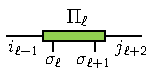
\includegraphics{figures/Pi_FactorizationLeft.pdf}} 
	\mathrel{\stackrel{\makebox[0pt]{\mbox{\normalfont\tiny prrLU}}}{\approx}}
		 \raisebox{-5mm}{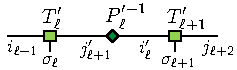
\includegraphics{figures/Pi_FactorizationRightPrime.pdf}} = \widetilde{\Pi}_\ell.
	\label{eq:Piapprox}
\end{equation}
In \prettyref{eq:ErrorPiIsErrorT} and \prettyref{eq:Piapprox} (and also \prettyref{fig:TCIalg}), $\Pi_\ell$ is reconstructed from the current set of local pivots $\mI_{\ell -1}$ and $\mJ_{\ell +2}$; $\widetilde{\Pi}_\ell$ is its approximation through prrLU. \prettyref{eq:ErrorPiIsErrorT} allows us to define a error concept consistent along the TT chain ($\forall \ell$), granting the TCI algorithm of a form error control. In fact, step $(c)$ in \prettyref{fig:TCIalg} is performed until the \textit{error} $\bigl| \Pi_\ell - \widetilde{\Pi}_\ell\bigr|_{i_{\ell-1}\sigma_\ell \sigma_{\ell +1} j_{\ell +2 }}$ is below a fixed tolerance $\varepsilon$. Minimizing the local error means, according to \prettyref{alg:prrLU} and the \textit{maxvol principle} \cite{Dolgov2020}, searching for the largest elements of the tensor $\bigl| \Pi_\ell - \widetilde{\Pi}_\ell\bigr|$, adding new pivots that yield the largest improvement to the local accuracy according to the $\|\cdot \|_{\infty}$ norm. The TCI routine is stopped when the condition $\bigl| \Pi_\ell - \widetilde{\Pi}_\ell\bigr| < \tau_{\Pi}$ is met $\forall \ell \in \{1,\dots,\mL\}$, for the minimal set of pivots possible and a fixed local tolerance $\tau_{\Pi}$. The last equality in \prettyref{eq:ErrorPiIsErrorT} in not trivial (cf. Ref.~\cite{Fernandez2024}) and allows to relate the local error $\bigl| \Pi_\ell - \widetilde{\Pi}_\ell\bigr|$ to the accuracy of the global approximation $\widetilde{T}$.

The TCI representation is defined by the selected lists $\mI_\ell$ and $\mJ_\ell$ $\forall \ell$, so an accurate interpolation amounts to optimizing this selection. The TCI routine, as mentioned at the beginning of this work, belongs to the class of ``active machine learning'' algorithms \cite{Settles2012}, as it tries to uncover the low-rank structure of a given tensor $\mT$ by actively requesting configurations that will better improve its MPS unfolding. Similar to other machine learning (ML) methods, different strategies exist to improve the modelling of our ``data set'' (e.g. for ML: data augmentation, weighting, prompt engineering etc.).
In our case, alongside the local pivot searching strategies -- \textit{rook search}, \textit{block rook search} and \textit{full search} -- other techniques exist to improve the global approximation of our tensor. The 2-site TCI can be run in \textit{reset mode} or \textit{accumulative mode}. The former recomputes the full lists $\mI_\ell$ and $\mJ_{\ell+1}$ at each prrLU step of the TCI routine, while the latter only adds new pivots to the alredy-existing local lists $\mI_\ell$ and $\mJ_{\ell+1}$. This allows us to discard sub-optimal pivots that were inserted in the pivots lists during the initial exploration of the configuration space, necessary to avoid the pivot matrices $P$ becoming singular. \textit{Global pivot proposals}, similar to multi-start approaches in ML \cite{Loshchilov2017}, allows the user to incorporate prior information about the tensor $\mT$ through a clever choice of the initial configurations $\boldsymbol{\hat  \sigma}$ (see \prettyref{fig:TCIalg}$.a$), such that all the relevant regions of configuration space are explored.

The above techniques all try to target TCI \textit{ergodicity} issues that arise in different implementations. Although most common TCI applications don't require any further expedient on top of the ones we just mentioned, as we will understand in the rest of this work, there exist many other, especially if modelling very extreme-conditioned physical systems, that call for additional improvements. In particular, \textit{sparse or symmetric tensors} and \textit{narrow peaked multivariate} functions are the main weaknesses for TCI.

\begin{table}[htbp]
	\centering
	\renewcommand{\arraystretch}{1.2} 
	\small      % shrink the font a bit (optional)
	\setlength{\tabcolsep}{4pt}  % tighter column separation (optional)
  
\begin{adjustbox}{max width=\textwidth} 
	\begin{tabular}{|c|c|c|c|c|}
	\hline 
	action & \multicolumn{2}{c|}{variant} & calls to $\mT_{\boldsymbol{\sigma}}$ & algebra cost\tabularnewline
	\hline 
	\hline 
	\multirow{4}{*}{iterate} & rook piv. & 2-site & $\order(\chi^{2}dn_{\text{rook}}\mL)$ & $\order(\chi^{3}dn_{\text{rook}}\mL)$\tabularnewline
	\cline{2-5} \cline{3-5} \cline{4-5} \cline{5-5} 
	 & full piv. & 2-site & $\order(\chi^{2}d^{2}\mL)$ & $\order(\chi^{3}d^{2}\mL)$\tabularnewline
	\cline{2-5} \cline{3-5} \cline{4-5} \cline{5-5} 
	 & full piv. & 1-site & $\order(\chi^{2}d\mL)$ & $\order(\chi^{3}d\mL)$\tabularnewline
	\cline{2-5} \cline{3-5} \cline{4-5} \cline{5-5} 
	 & full piv. & 0-site & 0 & $\order(\chi^{3}\mL)$\tabularnewline
	\hline 
	achieve full nesting & \multicolumn{2}{c|}{} & $\order(\chi^{2}d\mL)$ & $\order(\chi^{3}d\mL)$ \tabularnewline
	\hline 
	add $n_{p}$ global pivots & \multicolumn{2}{c|}{} & $\order\bigl((2\chi+n_{p})n_{p}\mL\bigr)$ & $\order\bigl((\chi+n_{p})^{3}\mL\bigr)$\tabularnewline
	\hline 
	\multirow{3}{*}{compress tensor train} & \multicolumn{2}{c|}{SVD} & \multirow{3}{*}{0} & \multirow{3}{*}{$\order(\chi^{3}d\mL)$}\tabularnewline
	\cline{2-3} \cline{3-3} 
	 & \multicolumn{2}{c|}{prrLU} &  & \tabularnewline
	\cline{2-3} \cline{3-3} 
	 & \multicolumn{2}{c|}{CI} &  & \tabularnewline
	\hline 
	\end{tabular}
\end{adjustbox}

\caption{Computational cost of the main TCI routines. Full nesting routines are useful to restore interpolation properties for our Tensor Train approximation. Rook pivoting and full pivoting are different possible choices for the pivot search in prrLU/CI subroutines. $n_{rook}$ corresponds to the maximum number of rook search moves necessary to find an optimal local pivot ($n_{\text{rook}} < 5$ for most applications). The table is taken directly from Ref. \cite{Fernandez2024}.}
\label{tab:cost}
\end{table}	

Tensor Cross Interpolation, as the $\mL$-dimensional extension of CI, conserves its compression properties. The number of elements of $\mT$ necessary for its TT decomposition is limited to the $\bsigma$ configurations obtained out of concatenation of the pivots in the \textit{pivot lists} -- $\mI_\ell$,$\mJ_{\ell +1}$ $\forall \ell$. Hence, the approximation is systematically controlled by $\chi$, where $\chi = \max_{\ell} \chi_\ell$ is the \textit{rank} of the tensor $\mT$ with $\chi_\ell = \dim \mI_\ell = \dim \mJ_{\ell +1}$ rank of the local pivot matrix $P_\ell$. As a consequence, the resources necessary to perform TCI scale strongly with $\chi$.

The number of function calls necessary for the MPS unfolding $\widetilde{\mathcal{T}}$ of $\mathcal{T}$ is $\order (\chi^2d^2\mathcal{L})$ compared to the $d^\mathcal{L}$ ($= |\text{Ind}\left(\mT\right)|$) of its SVD counterpart, where $d$ is the configuration space dimension. Such an exponential advantage is obtained by fully specifying only $\order (\chi^2\mathcal{L})$ number of \textit{pivots} from the original tensor. The algebra cost ($\sim$ computational time) of the algorithm scales as $\order (\chi^3d^2\mathcal{L})$. Table \ref{tab:cost} summarises the scaling of the core TCI routines implemented in the \texttt{TensorCrossInterpolation.jl} library \cite{TensorCrossInterpolation.jl}. As illustrated in Example \ref{ex:Ldimfunc}, these scalings underscore the pronounced memory efficiency inherent to TCI.
\begin{example}[$\mL$-dimensional function] Let us consider the following $\mL$-dimensional function, inspired by \cite{Fernandez2024}

\begin{equation}
	f(\boldsymbol{x}) = 
   \frac{2^\mL}{1 + 2 \sum^\mL_{\ell=1} x_\ell} .
   \label{eq:Ldimfunc}
\end{equation}

Such a continuous function can be numerically represented by a tensor $\mathcal{F}_{\bsigma}$ through grid discretization over a preferred domain. For this exercise, we take a 61 point Gauss-Kronrod type of grid, over the $[0,1]^\mL$ hypercube. What this means in practice is that $\mathcal{F}_{\bsigma} \in \mathds{R}^{d_1\times\dots\times d_\mL}$ \footnotemark\; and $\dim I_i = d = 61$. The TCI approximation of $\mathcal{F}_{\bsigma}$, namely $\widetilde{\mathcal{F}}_{\bsigma}$, is obtained through a limited number of calls to the original function $f(\boldsymbol{x})$, as depicted in \prettyref{fig:TCIscaling} below. 

\footnotetext{From this point onward, $\mF$ will refer to the tensor discretization of a continuous function, while $\mT$ will be the notation for a generic $\mL$-dimensional tensor.}

\prettyref{fig:TCIscaling} documents the reduced memory footprint required from the TCI representation of functions up to 20 dimensions. Exponential scaling of memory requirements, necessary to store the total $61^\mL$ number of tensor elements of $\mathcal{F}_{\bsigma}$, is replaced by a $\order \bigl(\chi^2\bigr)$ scaling. Moreover, as one can understand from the bottom right plot in \prettyref{fig:TCIscaling}, out of the total $61^2$ ($\mL=2$) Gauss-Kronod grid points, only $49$ are actually required for a nearly optimal approximation of $f$, therefore limiting the bond dimension $\chi$ of our tensor train to $\chi = 7$ and with that the number of total stored parameters. 
\begin{figure}[ht!]
		\centering
		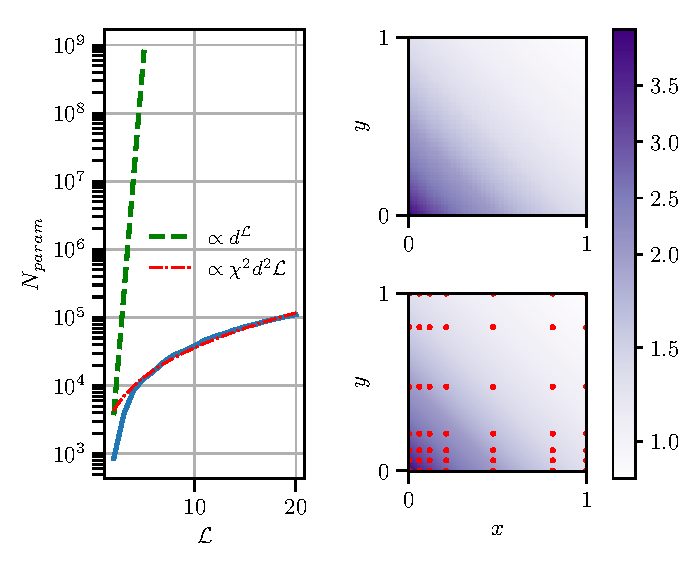
\includegraphics[width=0.9\textwidth]{figures/TCI_memory_scaling+heatmap.pdf}
		\caption{TCI approximation of $f(\boldsymbol{x})$ in \prettyref{eq:Ldimfunc} after discretization on a $\mL$-dimensional 61 point Gauss-Kronod grid. \textit{On the left}: number of total floating point elements stored in the compressed tensor $\widetilde{\mathcal{F}}_{\bsigma}$ as a function of $\mL$ (blue line). The ``worst-case-scenario'' scaling $d^\mL$ and the theoretical scaling $\order (\chi^2d^2\mathcal{L})$ are also represented (green and red dashed line, respectively). \textit{Top right:} heatmap of the $\mL = 2$ approximation $\widetilde{\mathcal{F}}_{\bsigma}$ over the $61\times61$ Gauss-Kronod grid, subset of $[0,1]\times[0,1]$, with absolute tolerance $\epsilon = 10^{-8}$. \textit{Bottom right:} heatmap of the $\mL = 2$ original function  $f(\boldsymbol{x})$ over the domain $[0,1]\times[0,1]$. The red dots represent the location of the \textit{pivot} values for the TCI approximation above.
		}
		\label{fig:TCIscaling}
	\end{figure}
\label{ex:Ldimfunc}
\end{example}

TCI is not only useful for function approximation. A very obvious application of TCI is the computation of integrals in high-dimensional spaces. Detailed examples of this particular usage of TCI are provided in Ref. \cite{Fernandez2022, Fernandez2024, Dolgov2020}. TCI-based integration outperform Monte-Carlo and quasi-Monte-Carlo methods in many occasions and the reasons behind it are diverse. 

Consider, for example, the following integral
\begin{equation}
	I \equiv \int d\boldsymbol{x} \ f(x_1,\dots,x_\mL),
	\label{eq:LdimIntegral}
\end{equation}
which can be approximated as a Riemann sum,
\begin{equation}
	I \approx \sum_{\bsigma} \mathcal{F}_{\bsigma}  ,\quad \; \mathcal{F}_{\bsigma} = f(\boldsymbol{x}(\bsigma))\;
	\label{eq:LdimapproxIntegral}
\end{equation}
where $\boldsymbol{x}(\bsigma)$ is our discretization grid (cf. Example \ref{ex:Ldimfunc}). If we decide to perform TCI unfolding of our numerical tensor $\mathcal{F}_{\bsigma}$ before the integration, \prettyref{eq:LdimapproxIntegral} then reads\footnotemark
\begin{equation}
	\sum_{\bsigma} \mathcal{F}_{\bsigma} \approx \prod_{\ell=1}^\mL \sum^{d_\ell}_{\sigma_\ell = 1} T^{\sigma_\ell}_\ell P^{-1}_\ell
	\label{eq:LdimTCIIntegral}
\end{equation}
replacing one $\mL$-dimensional integral by $\chi^2\mL$ exponentially easier 1-dimensional integrals. Moreover, if the rank of the MPS unfolding of the integrand remains roughly constant as the number of dimensions increases, then the advange provided by TCI increases exponentially. Given the numerical simplicity of the algebra operations in \prettyref{eq:LdimTCIIntegral}, the bottleneck of integration operations is limited to finding the right TCI approximation of the integrand, bounding the parameter scaling to a \textit{polynomial} cost of $\order (\chi^2d\mathcal{L})$. 

\footnotetext{$P$ and $T$ slices are here considered as ($\sigma_\ell$-dependent) matrices. Summation over common indices is therefore implied. $P_{\mL} = [1]$.}

The above achievement of TCI relies on the following property of continuous functions:
\begin{definition}
	A function $f$ is {\normalfont \textbf{almost separable}} \cite{Fernandez2024} or {\normalfont \textbf{$\boldsymbol{\varepsilon}$-factorizable}} \cite{Fernandez2022} if its tensor representation $\mathcal{F}$ is low-rank.
	\label{def:separfunc}
\end{definition}

For this class of functions the numerical advantage of TCI integration over more standard approaches -- like Monte Carlo sampling -- is remarkable (cf. $1/N_{\text{eval}}^4$ vs. $1/\sqrt{N_{\text{eval}}}$ convergence for $N_{\text{eval}}$ function evaluations in Fig. 2 of Ref. \cite{Fernandez2024}). In addition, TCI does not suffer from the \textit{``sign problem''} \cite{Loh1990} of Monte Carlo methods, \textit{i.e.} slow convergence of the integral error with the number of samples when ingrating over strongly oscillating functions. On the other hand, TCI performs well even when integrating functions oscillating simultaneously on very different scales. The limiting factor of TCI (rank of the $\varepsilon$-factorization) is entirely orthogonal
to that of sampling methods.

If the user intends to employ TCI purely to perform integrations, the definition of an \textit{environment-aware error} (from \prettyref{eq:ErrorPiIsErrorT} and \prettyref{eq:LdimTCIIntegral}) might turn out to be very useful. It is defined as

\begin{gather}
	\nonumber\bigl[\varepsilon^{\text{env}}_\Pi\bigr]_{i_{\ell-1}\sigma_\ell \sigma_{\ell +1} j_{\ell +2 }}\equiv |L_\ell R_\ell| \bigl[\varepsilon_\Pi\bigr]_{i_{\ell-1}\sigma_\ell \sigma_{\ell +1} j_{\ell +2 }} \\
	L_\ell = \prod_{\bar{\ell}=1}^{\ell -1} \sum^{d_{\bar{\ell}}}_{\sigma_{\bar{\ell}} = 1} T^{\sigma_{\bar{\ell}}}_{\bar{\ell}} P^{-1}_{\bar{\ell}} \quad R_\ell = \prod_{\bar{\ell}=\ell +2}^{\mL} \sum^{d_{\bar{\ell}}}_{\sigma_{\bar{\ell}} = 1}  P^{-1}_{\bar{\ell}-1}T^{\sigma_{\bar{\ell}}}_{\bar{\ell}}.
	\label{eq:envError}
\end{gather}

The environment error function $\varepsilon^{\text{env}}_\Pi$, by readjusting 
Substituting the usual definition of local  error $\varepsilon_\Pi$ ot be the error of the inegrand, allows the TCI routine to be more integral-focused, outperforming the standard implementation when it comes to integral error convergence. By selecting pivots not only based on the absolute value of the integrand but also taking into account a specific point's volume contribution to the integral,  $\varepsilon^{\text{env}}_\Pi$ allows for more precise computations of complex integrals particularly for multi-scaled functions \cite{Fernandez2022}.   

\subsection{The Quantics Representation: QTCI}
TCI is a powerful tool that can be used ``out-of-the-box'' for most applications. The standard implementation however lacks the capabilities of reaching very high resolutions for the approximatino of function of lower dimensions. Let us consider \prettyref{fig:TCIscaling} in Example \ref{ex:Ldimfunc}: one might have noticed that the plot depicting the TCI approximation of \prettyref{eq:Ldimfunc} shows some subtle visual imperfections. These imperfections arise naturally when discretization errors become dominant in our TCI representation. A naive solution to this issue would be to increase the number of total grid points $d\times d$ used to discretize our 2D function. Despite solving our discretization troubles, such an easy fix will make the number of grid points $d$ the main contributor to TCI scaling, reducing the compression capabilities of the TT unfolding (e.g. for our specific example with $\mL = 2$ and, let's say, $d=1000$ grid points we would obtain a 2-sited MPS with site dimension $1000$). 

Given a function $f(\boldsymbol{x})$ which we intend to resolve at very high resolution -- or more ambitiously at \textit{superhigh resolution} -- the \textit{quantics tensor representation} could turn out to be very advantageous. Quantics representation has been a standard approach -- not limited to TT approximations -- to target resolution issues, well-established in the literature \cite{Oseledets2009, Khoromskij2011, Hiroshi2023, Takahashi2025, Murray2024, Ritter2024}. Applications revolving around this type of representation are quite diverse in the many-body physics community, ranging from computations of correlation functions for quantum many body systems \cite{Hiroshi2023} to diagrammatic non-equilibrium many-body Green’s function-based calculations \cite{Murray2024} and compression of imaginary-time propagators in the Frobenious norm \cite{Takahashi2025}.

Discretization errors are often a consequence of poor scaling of our numerical approximation tool or of a suboptimal grid choice. While the former is definitely not an issue in the context of TCI \cite{Fernandez2024}, the latter can definitely be better addressed.

Given a function of $\mathcal{N}$ variables $f(\boldsymbol{x})$ we discretize each variable through a dyadic grid with \(M=2^{\mR}\) points per variable, 
\begin{equation}
	x_n(m_n) = (x_{n,\text{max}} - x_{n,\text{min}})\frac{m_n}{2^{\mR}} + x_{n,\text{min}}
	\label{eq:quanticsGrid}
\end{equation}
where each index \(m_n\in\{0,\dots,M-1\}\) is written in binary form with $\mR$ bits as 
\begin{equation}
	m_n(\bsigma_n)  = m_n(\sigma_{n1},\dots,\sigma_{n\mR})=\sum_{r=1}^{\mR}\sigma_{nr}\,2^{\,\mR-r},\quad 
\quad \sigma_{nr}\in\{0,1\},
\label{eq:quanticsRepr}
\end{equation}
so that the \(\mathcal{N}\)-variate function \(f\) is represented by the binary tensor \(\mathcal{F}_{\boldsymbol{\sigma}}:=f\!\bigl(x_1(\bsigma_1),\dots,x_\mN(\bsigma_\mN)\bigr)\) on such a grid \cite{Khoromskij2011, Hiroshi2023}.

A well-defined tensor \(\mathcal{F}_{\boldsymbol{\sigma}}\) requires us to unambiguously specify the \textit{order} of the tensor indices so that an MPS representation can be constructed These aer multiple possible orderings
\begin{itemize}
	\item \textit{natural ordering}: $\mathcal{F}_{\boldsymbol{\sigma}} \equiv \mathcal{F}_{(\sigma_{11},\dots,\sigma_{1\mR},\sigma_{21},\dots,\sigma_{2\mR}, \dots\dots,\sigma_{\mN1},\dots,\sigma_{\mN\mR})}$ combining dimensions;
	\item \textit{interleaved ordering}: $\mathcal{F}_{\boldsymbol{\sigma}} \equiv \mathcal{F}_{(\sigma_{11},\dots,\sigma_{\mN1},\sigma_{12},\dots,\sigma_{\mN2}, \dots\dots,\sigma_{1\mR},\dots,\sigma_{\mN\mR})}$ combining scales;
	\item \textit{fused ordering}: $\mathcal{F}_{\tilde \bsigma} \equiv \mathcal{F}_{({\tilde \bsigma}_{1},\dots,{\tilde \bsigma}_{\mR})}$ fusing scales, where ${\tilde \bsigma}_r = \sum_{n=1}^\mN 2^{n-1}\sigma_{nr}$.
\end{itemize} 
Once the \textit{index ordering} is established, cross interpolation of the tensor \(\mathcal{F}_{\boldsymbol{\sigma}}\) yields a TT approximation of our initial function $f$. 

Combining TCI with the quantics representation allows us to represent a given function $f$ through an MPS and resolve it up to a scale of order $1/2^{\mR}$; we will name this routine \textit{Quantics Tensor Cross Interpolation} or \textit{QTCI}. 

QTCI constructs the local tensors \(T^{\sigma_\ell}_\ell\) and \(P^{-1}_\ell\) with a cost of \(\order(\mL d\chi^{2}) = \order( \chi^2 d \log M)\), similar to TCI, i.e. linear in the number of bits $\mR$ and logarithmic in the grid size (recovering Khoromskij’s \(O(d\log n)\) scaling \cite{Khoromskij2011}), where $\mL = \mN \mR$ or $\mL = \mR$ depending on the index ordering choice. On the other hand, because the mesh width is \(\Delta=2^{-R}\), analytic \(f\) satisfy a spectral
error bound
\begin{equation}
	\|f-\tilde f_R\|_\infty\;\le\;C\,e^{-cR}=C\,\Delta^{c/\ln 2},
\end{equation}
so that the discretization error decays exponentially with $\mR$ while storage and CPU time grow only linearly with it \cite{Khoromskij2011, Lindsey2024}.

Interleaving (fusing) the bits as \(\sigma_{\ell(n,r)}\) -- where $\ell = n + (r-1)\mN$ ($\ell = r$) -- arranges (fuses) all sites that resolve the \emph{same} length‑scale \(2^{-r}\) next to (with) one another. Whenever cross‑scale correlations are weak this ordering yields a tensor‑train (TT) of small, \(\mR\)-independent rank \(\chi\) \cite{Hiroshi2023, Khoromskij2011}. QTCI has no problem uncovering such an underlying structure, discarding the weak entanglement betweeen different scales. Let us discuss this further in the following example. 

\begin{example}[2D scale separated function]
	Consider the following 2D function 
	\begin{equation}
		\begin{aligned}
		f(x,y) &= \exp(-0.4(x^2 + y^2)) + 1 + \sin(xy)\exp(-x^2)\\
		&+ \cos(3xy)\exp(-y^2) + \cos(x + y)\\ 
		&+2^{-4}\cos(2^{-4}(0.2x - 0.4y))+
          2^{-8}\cos(2^{-4}(-0.2x + 0.7y))
		\end{aligned}
		\label{eq:scaleSepFunc}
	\end{equation}
	The $f$ might present a very high level of scale separation, where each individual function scale, of order $\order(1)$, $\order(1/2^4)$ and $\order(1/2^8)$ respectively, sees the rest of the function either as a summing constant or as some irrelevant small-magnitude noise. We may expect that performing a QTCI compression of this function, with interleaved ordering, would render a low-ranked TT, given this separation. The level of entanglement between different bit bipartitions can give us an intuition of the amount of scale disconnection present in the function. 
	
	An entanglement measure can be achieved through the \textbf{Von Neumann} -- or \textbf{entanglement entropy} $S$. Given a generic tensor representation of the form $F_{\sigma_1\dots\sigma_\mL}$, the Von Neumann entropy at site $\ell$ can be evaluated through singular value decomposition (SVD) of the matrix 
	
	\begin{equation}\rho_\ell = \rho_{(\sigma_1\dots\sigma_\ell),(\sigma'_1\dots\sigma'_\ell)} = \sum_{\sigma_{\ell +1}\dots\sigma_\mL}F_{(\sigma_1\dots\sigma_\ell),(\sigma_{\ell+1}\dots\sigma_\mL)}F^\dag_{(\sigma_{\ell+1}\dots\sigma_\mL),(\sigma'_1\dots\sigma'_\ell)}.\end{equation}
	The  singular values of $\rho_\ell$, namely $s_\ell$, can then be used, after normalisation, to calculate the local Von Neumann entropy 
	\begin{equation}
		S_\ell = - \sum_{\alpha=1}^{\chi_\ell} s_\ell^2 \log s_\ell^2
	\end{equation}
	as entanglement measure between the bipartions $(\sigma_1\dots\sigma_\ell)$ and $(\sigma_{\ell+1}\dots\sigma_\mL)$ of the system.
	
Since bits $\ell = 2(r-1)$ and $\ell = 2(r-1) + 1$ (interleaved representation with  $\mN = 2$) resolve scale $2^{-r}$ of our function, entanglement measure around these sites can give us an intuition of the amount of information that needs to be propagated from scale $2^{-r}$ to the other scales for a correct TT representation of $f$. \prettyref{fig:QTCIEntanglement} depicts this entanglement measure for the QTCI compression with $\mR = 10$ of $f(x,y)$ in \prettyref{eq:scaleSepFunc} and of $\texttt{rand(}x,y\texttt{)}$, that generates random noise. $\texttt{rand(}x,y\texttt{)}$ is the perfect example of non-compressible function: no hidden low-rank structure and absolutely no scale separation. In the case of $f$ we can observe very low entanglement for all the different bit bipartions, proving once agan its scale separation. On the contrary, the random noise function is strongly entangled along its whole MPS chain and the entire discretized tensor is necessary to represent it as an MPS, such that no compression is achieved by (Q)TCI. Accordingly, the bond dimensions are much larger for \texttt{rand()} than for $f(x,y)$
	
\begin{figure}[htbp]
		\centering
		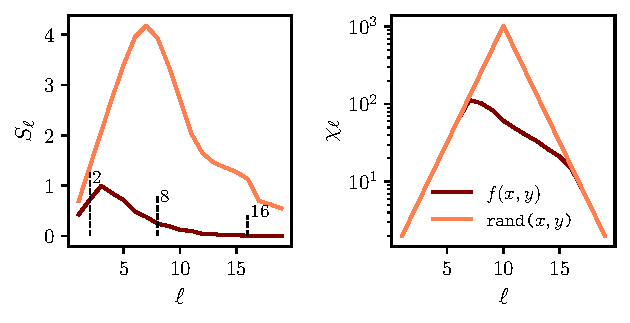
\includegraphics[width=0.9\textwidth]{figures/QTCI_ent_entropy+bonddims.pdf}
		\caption{ \textit{Left:} entanglement entropy per site $S_\ell$ vs site $\ell$ for the function of \prettyref{eq:scaleSepFunc} and a 2D random noise function. The vertical dashed lines indicate the bonds where the bits $(\sigma_{1r'}, \sigma_{2r'})$, for $r' \in [1,4,8]$, are next to the bipartition cut. \textit{Right:} bond dimension per site $\chi_\ell$ for the same two functions.}
		\label{fig:QTCIEntanglement}
	\end{figure}
\end{example}
When computing numerically with multivariate functions, one must usually balance two opposing aims: faithfully capturing the function's detail and minimising the memory required for it. Employing the quantics representation together with TCI compression, however, allows us to realise \emph{high resolutions} (\(\Delta\!\to\!0\)) at limited computational cost, making QTCI the
method of choice whenever scale-separation permits a small TT rank.

\subsection{\texttt{TensorCrossInterpolation.jl} library}

In the previous sections we introduced technical details and different applications of the TCI and QTCI algorithms. As briefly mentioned, all of the examples we presented rely on a $\julia$ implementation of the algorithm, namely \texttt{TensorCrossInterpolation.jl} \cite{TensorCrossInterpolation.jl, tensor4all.org}.  We will not dive into this details of the library however, as reference for the rest of the work, we will mention its main functionality: the \texttt{crossinterpolate2} function.

\texttt{crossinterpolate2}, described in the Listing \ref{code:crossinterpolate2} below, performs TCI of a given numerical function \texttt{f}; in our context, \texttt{f} is either represented by the discretized version of a multi-variate continuous function -- $f(\boldsymbol{x}(\bsigma))$ -- or by any tensor-like numerical function -- $\mF_{\bsigma}$. Given the definition of our tensor $\mF_{\bsigma}$ as a \texttt{function} type, we can understand that its elements don't need to be known and stored beforehand. 
The output of the computation is an object containing the site tensors of the TT-unfolding, together with the lists of pivots necessary to realize the cross approximation.

\begin{lstlisting}[language = julia, caption={Main TCI routine of the \texttt{TensorCrossInterpolation.jl} library \texttt{crossinterpolate2}. The details of each input variable are described in the relative inline comments.}, label={code:crossinterpolate2}]
 function crossinterpolate2(
  ::Type{ValueType},        # Return type of f, usually Float64 or ComplexF64
  f,                        # Tensorized function of interest: $\color{Maroon} f(\boldsymbol{x}(\bsigma))$ or $\color{Maroon} \mF_{\bsigma}$
  localdims::Union{Vector{Int},NTuple{N,Int}},  # Local dimensions $\color{Maroon} (d_1, \ldots, d_\mL)$
  initialpivots::Vector{MultiIndex};  # List of initial pivots $\color{Maroon} \{\hat\bsigma\}$. 
  									  # Default: $\color{Maroon} \{(1, \ldots, 1)\}$
  tolerance::Float64,       # Global error tolerance $\color{Maroon} \tau$ for TCI. Default: $\color{Maroon} 10^{-8}$
  pivottolerance::Float64,  # Local error tolerance $\color{Maroon} \tau_{\Pi}$ for prrLU. Default: $\color{Maroon} \tau$
  maxbonddim::Int,          # Maximum bond dimension $\color{Maroon} \chi_{\max}$. Default: no limit
  maxiter::Int,             # Maximum number of half-sweeps. Default: $\color{Maroon} 20$
  pivotsearch::Symbol,      # Full or rook pivot search? Default: :full
  normalizeerror::Bool,     # Normalize $\color{Maroon} \varepsilon$ by $\color{Maroon} \max_{\bsigma \in \mathrm{samples}} \mF_{\bsigma}$? Default: true
  ncheckhistory::Int        # Convergence criterion: 
  							# $\color{Maroon} \varepsilon_{n_{\textrm{iter}}} < \varepsilon$ for how many iterations? Default: 3
) where {ValueType,N}
\end{lstlisting}


\section{QTCI approximation of functions with narrow peaks}
\label{sec:TCIFallbacks}
Sparse or symmetry-constrained tensors, and--more relevant here--multivariate
functions that contain a few sharp local peaks, expose two latent weaknesses of standard TCI.
First, the informative regions of the configuration space occupy only a tiny fraction of the full domain; random or purely local pivot searches can miss them, revealing TCI's \emph{ergodicity} problem.
Second, fitting the entire (mostly trivial) domain with a \emph{single} tensor train forces one global bond dimension, even though different parts of the domain in fact require widely different ranks. The result is often an over-ranked representation of the function, which mostly traslates to an unnecessary increase in memory costs.

To illustrate these limitations—and to motivate the distributed strategy developed in the following chapters—we introduce a minimal variant of TCI tailored to sharply localised functions.


\subsection{A ``naive'' solution}

\textit{Ergodicity} problems render TCI -- and QTCI as well -- a deficient tool when we attempt to approximate functions with very local and sharp features. 
This can be solved by \textit{global pivot insertion}, where additional sampling points $\hat{\bsigma}$ are inputted by an external source. Proposing clever initial configurations $\hat{\bsigma}$ (see \prettyref{fig:TCIalg}) to the TCI routine -- similar to prompt engineering in deep learning algorithms -- can help TCI uncover all the relevant features of the function of interest. The main weakness of this approach is that the target function we intend to TCI compress might not be known \emph{a priori}, so no information can be used to improve its approximation.
Let us consider the following function 
\begin{gather}
		f(\boldsymbol{r}) ={\color{mymagenta} \underbrace{A_1\, e^{-\frac{(\boldsymbol{r} - \boldsymbol{r}_1)^2}{2\sigma^2_1}} \sin(k_1\boldsymbol{r})}_{f_1(\boldsymbol{r})}} + {\color{green} \underbrace{A_2\, e^{-\frac{(\boldsymbol{r} - \boldsymbol{r}_2)^2}{2\sigma^2_2}} \sin(k_2\boldsymbol{r})}_{f_2(\br)}},
		\label{eq:localFunc}
\end{gather}
	where
\[
\begin{gathered}
	\boldsymbol{r} = (x,y), \quad \boldsymbol{r}_{1/2} = \pm( 0.5, 0.5),\\[6pt]
	A_1 = 10^{3}, A_2 = 10^6, \quad \sigma_1 = 10^{-1}, \sigma_2 = 10^{-3}, \quad k_1 = 10^4, k_2 = 10^3. 
\end{gathered}
\]
\begin{figure}[ht!]
	\centering
	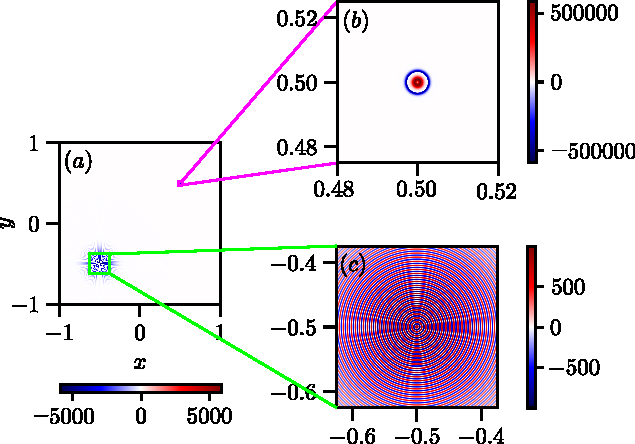
\includegraphics[width=0.7\textwidth]{figures/Heatmap_localised_func.pdf}
	\caption{ $(a)$ Heatmap of the function $f(\boldsymbol{r})$ within the domain $[0,1]^2$. Zoomings into the enviroment of $(b)$ $\br_1$ and $(c)$ $\br_2$, which are the peak positions of ${\color{mymagenta} f_1}$ and ${\color{green} f_2}$, respectively. \prettyref{eq:localFunc}.}
	\label{fig:localFunc}
\end{figure}

$f(\boldsymbol{r})$ is composed by two, almost indipendent terms, with very different absolute scales. $f_1(\boldsymbol{r})$ has wider support but it smaller in absolute value and more slowly oscillating, whereas $f_2(\boldsymbol{r})$ is quickly oscillating but more localised and of larger absolute value. After quantics discretization, the tensor $f(\boldsymbol{r}(\bsigma)) = \mF_{\bsigma}$ can be TCI compressed to $\widetilde{\mF}_{\bsigma}$. 

The absolute quality of the local approximation can be measured through 
\begin{equation}
	\varepsilon_{\text{log}}(\boldsymbol{r}(\bsigma)) = \log_{10}\left|\mF_{\bsigma} - \widetilde{\mF}_{\bsigma}\right|, \quad \boldsymbol{r}(\bsigma) \in [0,1]^2
	\label{eq:logTCIerror}
\end{equation}
where a smaller value indicates better precision. 
We show this error measure in the \textit{top central} plot in \prettyref{fig:errorLocalFunc}, for a QTCI of $f$ with $R=20$, desired absolute tolerance $\tau = 10^{-7}$ and fused quantics index ordering. The image suggests that -- as expected from \prettyref{fig:localFunc} -- most of the function domain is easy to represent, while the computational effort is focused around the centers of our local features $\boldsymbol{r}_1$ and $\boldsymbol{r}_2$. Dividing the domain into computationally simple and complex subdomains -- or \textit{patches} -- could benefit the overall cost and, to some degree, accuracy of the QTCI representation. Other arguments support this strategy, as follows. 

\begin{figure}[ht!]
	\centering
	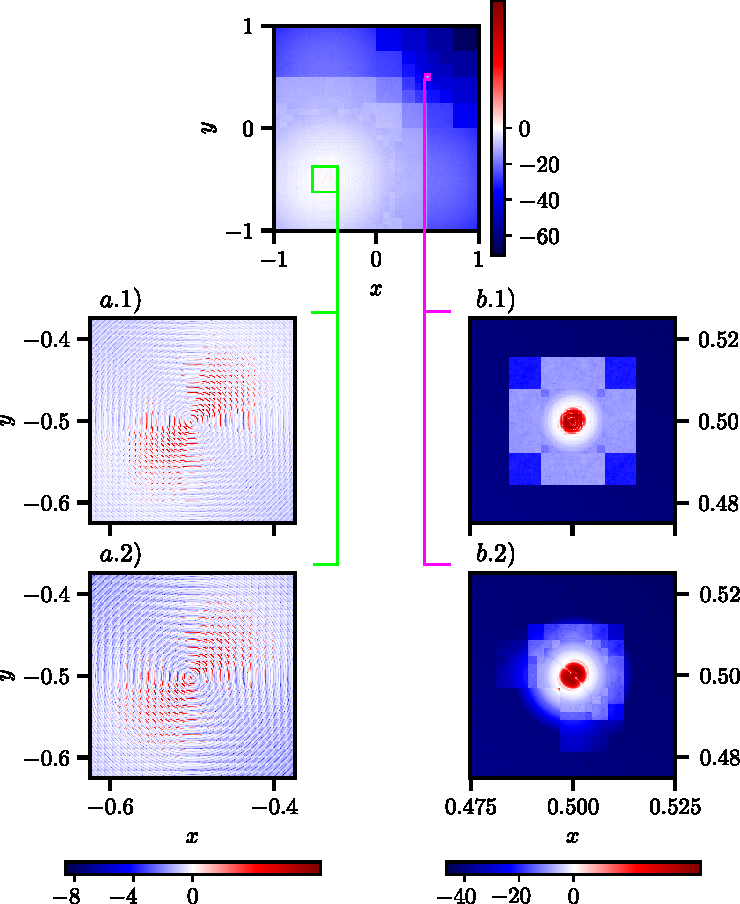
\includegraphics{figures/Error_heatmap_localFunc.pdf}
	\caption{Logarithmic error $\varepsilon(\boldsymbol{r}(\bsigma))$ for the QTCI representation $\widetilde{\mF}_{\bsigma}$ of $f(\boldsymbol{r})$ in \prettyref{eq:localFunc} (\textit{top}) with different zoomings (\textit{a-b.1}). Error measure of QTCI of $f$ \textit{limited} to the surrounding of $\boldsymbol{r}_1$ and $\boldsymbol{r}_2$ is also shown (\textit{a-b.2}). We refer to the main manuscript for further details. }
	\label{fig:errorLocalFunc}
\end{figure}

Given two tensors $A_{\bsigma}$ and 
$B_{\bsigma}$ on the same configuration space $\bsigma$, we define the element-wise sum tensor $S_{\bsigma} = A_{\bsigma} + B_{\bsigma}$ as the direct sum -- or partial direct sum -- of the two tensors. The same operation can be performed for Tensor Trains, by direct summing each site tensor (cf. \prettyref{sec:patchAlg} and Ref. \cite{Lee2018}). 
In our particular example, if we decide to approximate each summand $f_1(\boldsymbol{r})$ and $f_2(\boldsymbol{r})$ in \prettyref{eq:localFunc} with TTs -- $\widetilde{\mF}_1$ and $\widetilde{\mF}_2$ -- then 
\begin{equation}
	f(\boldsymbol{r}(\bsigma)) = \mF_{\bsigma} \approx \widetilde{\mF}_{1\bsigma} + \widetilde{\mF}_{2\bsigma} = \widetilde{\mF}^+_{\bsigma}
	\label{eq:localTermsSum}
\end{equation}
with negligible error, due to the independency of the two terms. \prettyref{fig:errorLocalFunc}, supports this argument. The first pair of plots \textit{(a.1)} and \textit{(b.1)} portray the error function of the QTCI approximation \textit{focused} on the support region of $f_1(\boldsymbol{r})$ and $f_2(\boldsymbol{r})$. The second pair \textit{(a.2)} and \textit{(b.2)}, on the other hand, measures the error for the QTCI approximations -- $\widetilde{\mF}_{2\bsigma}$ and $\widetilde{\mF}_{1\bsigma}$ -- \textit{limited} \footnotemark to the support of $f_1(\boldsymbol{r})$ and $f_2(\boldsymbol{r})$.

\footnotetext{When limiting the QTCI approximation, in order to produce results with similar resolution to the standard application, we reduce the number of bits to $\mR_1 = 17$ and $\mR_2 = 16$, while keeping the other parameters unchanged.}

We can observe a slight improvement in the local approximation error in the last row of plots compared to the first one. Whenever QTCI is constricted to each local feature of $f$ it is able to resolve the target with better precision. Nevertheless, the main advantage of this naive solution is not this small accuracy improvement \textit{per se}. 

The computational effort of this \textit{``divide and conquer''} variant of QTCI -- apart from being very well suited for parallelization -- frees the algorithm from the constraint of representing a single object, made of different independent components, using a single tensor train. The improvement in numerical resources requirement is non-negligible. The bond dimension development along the chains of the MPS unfoldings $\widetilde{\mF}_{\bsigma}$, $\widetilde{\mF}_{2\bsigma}$ and $\widetilde{\mF}_{1\bsigma}$ is a witness of that, as shown in \prettyref{fig:bondDimLocalFunc}. 

\begin{figure}[ht!]
	\centering
	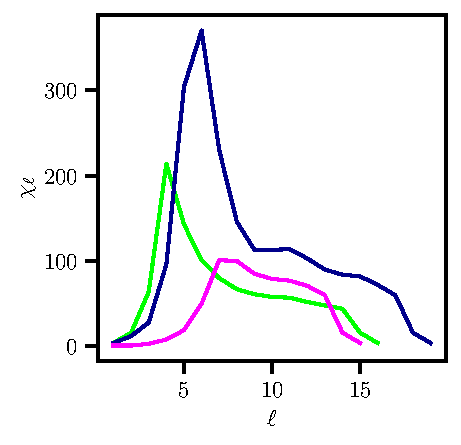
\includegraphics[width=0.7\textwidth]{figures/bonddim_localised_func+bonddim_patches.pdf}
	\caption{Bond dimension per-site of the TT unfolding of $f(\boldsymbol{r})$ (blue line) and of the TT unfoldings of ${\color{mymagenta}f_1(\boldsymbol{r})}$ and ${\color{green} f_2(\boldsymbol{r})}$ in \prettyref{eq:localFunc}, limited to their respective support. The respective Tensor Trains  $\widetilde{\mF}_{\bsigma}$, $\widetilde{\mF}_{1\bsigma}$ and $\widetilde{\mF}_{2\bsigma}$ are obtained through QTCI. }
	\label{fig:bondDimLocalFunc}
\end{figure}

The rank $\chi^+$ of the direct sum of MPSs -- $\widetilde{\mF}^+_{\bsigma}$ -- in \prettyref{eq:localTermsSum}, depends only linearly on the bond dimension of its addends, \textit{i.e.}

\begin{equation}
	\chi^+ = \chi_1 + \chi_2,
\end{equation}
where $\chi_1$, $\chi_2$ are the ranks of $\widetilde{\mF}_{1\bsigma}$ and $\widetilde{\mF}_{2\bsigma}$, respectively. 

Since $f_1$ and $f_2$ are resolved at markedly different scales, combining them still yields a pronounced drop in the overall bond dimension, despite the extra ranks introduced during the summation that produces the final tensor; as evidence of this, the total number of floating point parameters necessary for the two different implementations is 

\begin{equation}
	N_{\text{par}}(\widetilde{\mF}_{\bsigma}) \simeq 1.4 \times 10^6 > N_{\text{par}}(\widetilde{\mF}_{2\bsigma} + \widetilde{\mF}_{1\bsigma}) \simeq 5.6 \times 10^5.
	\label{eq:naiveLocalFuncMemorySave}
\end{equation}




